% Template for a Computer Science Tripos Part II project dissertation
\documentclass[12pt,a4paper,twoside,openright]{report}
\usepackage[pdfborder={0 0 0}]{hyperref}    % turns references into hyperlinks
\usepackage[margin=25mm]{geometry}  % adjusts page layout
\usepackage{graphicx}  % allows inclusion of PDF, PNG and JPG images
\usepackage{verbatim}
\usepackage{docmute}   % only needed to allow inclusion of proposal.tex
\usepackage{parskip}
\usepackage{listings}
\usepackage{todonotes}

\lstset{basicstyle=\ttfamily, breaklines=true}

\graphicspath{ {./images/} }

\newcommand{\quickwordcount}[1]{%
  \immediate\write18{texcount -1 -sum -merge -q #1.tex output.bbl > #1-words.sum }%
  \input{#1-words.sum}%
}

\raggedbottom                           % try to avoid widows and orphans
\sloppy
\clubpenalty1000%
\widowpenalty1000%

\renewcommand{\baselinestretch}{1.1}    % adjust line spacing to make
                                        % more readable

\begin{document}

\bibliographystyle{plain}


%%%%%%%%%%%%%%%%%%%%%%%%%%%%%%%%%%%%%%%%%%%%%%%%%%%%%%%%%%%%%%%%%%%%%%%%
% Title


\pagestyle{empty}

\rightline{\LARGE \textbf{Jiaxin Wang}}

\vspace*{60mm}
\begin{center}
\Huge
\textbf{A Recursive Recurrent Neural Network Decoder for Grammatical Error Correction} \\[5mm]
Computer Science Tripos -- Part II \\[5mm]
Emmanuel College \\[5mm]
\today  % today's date
\end{center}

%%%%%%%%%%%%%%%%%%%%%%%%%%%%%%%%%%%%%%%%%%%%%%%%%%%%%%%%%%%%%%%%%%%%%%%%%%%%%%
% Proforma, table of contents and list of figures

\pagestyle{plain}

\chapter*{Proforma}

{\large
\begin{tabular}{ll}
Candidate Number:   & -                       \\
Project Title:      & A Recursive Recurrent Neural Network \\
 & Decoder for Grammatical Error Correction \\
Examination:        & Computer Science Tripos -- Part II, 2022  \\
Word Count:         & \quickwordcount{diss}\footnotemark[1] \\
Code line count:    & - \\
Project Originator: & - \\
Supervisor:         & Dr Zheng Yuan, Dr Christopher Bryant
\end{tabular}
}
\footnotetext[1]{This word count was computed
by \texttt{detex diss.tex | tr -cd '0-9A-Za-z $\tt\backslash$n' | wc -w}
}
\stepcounter{footnote}


\section*{Original Aims of the Project}

-


\section*{Work Completed}

-

\section*{Special Difficulties}

-
 
\newpage
\section*{Declaration}

I, Jiaxin Wang of Emmanuel College, being a candidate for Part II of the Computer
Science Tripos, hereby declare that this dissertation and the work described in 
it are my own work, unaided except as may be specified below, and that the dissertation
does not contain material that has already been used to any substantial
extent for a comparable purpose.

\bigskip
\leftline{Signed [signature]}

\medskip
\leftline{Date [date]}

\tableofcontents

\listoffigures

\newpage
\section*{Acknowledgements}

-

%%%%%%%%%%%%%%%%%%%%%%%%%%%%%%%%%%%%%%%%%%%%%%%%%%%%%%%%%%%%%%%%%%%%%%%
% now for the chapters
\listoftodos

\pagestyle{headings}

\chapter{Introduction}

This project concerns my implementation of a \textit{recursive recurrent neural network} model (R\textsuperscript{2}NN) proposed by Liu et al. (2014) \cite{r2nn} This is to be integrated in a statistical machine translation (SMT) system to attempt the task of grammatical error correction. \todo[inline]{How well have you done?}

\section{Motivation}

Grammatical Error Correction (GEC) is the task of producing a grammatically correct sentence given a potentially erroneous text while preserving its meaning. The main motivation behind this task lies in its role in helping learners of a foreign language understand the language better. In addition, native speakers can make use of such GEC tools to avoid mistakes in their writing. Being an ESL (English as a second language) learner myself, I would like to investigate models that can be used for the task of GEC in English, and I hope that it can benefit people who may find GEC tools useful.


\section{Problem Overview}

The task of Grammatical Error Correction can be seen as a machine translation process, where the input is a text which may contain grammatical errors, and the output is an error-free text. This project uses a statistical machine translation (SMT) approach to solve GEC.

A recursive recurrent neural network (R\textsuperscript{2}NN) was proposed by Liu et al. (2014) \cite{r2nn} for SMT. The goal of this project is to implement the proposed model to be used for GEC. The model should aim to correct all types of errors, namely grammatical, lexical, and orthographical errors. Its performance will be evaluated against a baseline SMT system, Moses\cite{moses}.


\section{Related Work}
-

\chapter{Preparation}

\section{Starting Point}

This project is based on the idea presented in the paper \textit{A Recursive Recurrent Neural Network for Statistical Machine Translation} \cite{r2nn}. An R\textsuperscript{2}NN model was proposed, but the implementation details are not given in the paper.

The Part IB Computer Science Tripos course Artificial Intelligence\footnote{https://www.cl.cam.ac.uk/teaching/2021/ArtInt/} gives an introduction to neural networks and explains how forwarding and backpropagation works. Prior to this project I did not have any coding experience with neural networks. I have found it useful to follow the coding examples on PyTorch\footnote{https://pytorch.org/tutorials/} website.

An example SMT system is available on Moses\footnote{https://www.statmt.org/moses/?n=Moses.Baseline} website. It provides a detailed tutorial on how to install Moses, how to prepare corpus and how to train the SMT.


\section{Theory}

\subsection{SMT system}
A typical SMT system consists of four main components: The language model (LM), the translation model (TM), the reordering model and the decoder\cite{yuan2017phd}. The LM computes the probability of a given sequence being valid. The TM builds a translation table which contains mappings of words/phrases between source and target corpora. The reordering model learns about phrase reordering of translation. The decoder finds a translation candidate who is most likely to be the translation of the source sentence. In the task of GEC, this would be the most probable correction to the original erroneous sentence.

\todo[inline]{Level of detail?}


\subsection{Moses SMT}
The Moses baseline system uses KenLM as the language model. For the translation model, it uses GIZA++ to obtain a word alignment model. The model should be trained to produce a phrase table and associated scores. Reordering tables are also created during this process. Eventually, the Moses decoder will find the best translation candidate given input based on the scores it calculated in previous stages.

\subsection{Feedforward Neural Network}
A feedforward neural network consists of three parts: an input layer, one or more hidden layers, and an output layer. In a feedforward neural network, data only flows in one direction (forward) from input to output. Figure \ref{fig:fnn} shows an example of a feedforward neural network with one hidden layer.

\begin{figure}[ht]
\centering
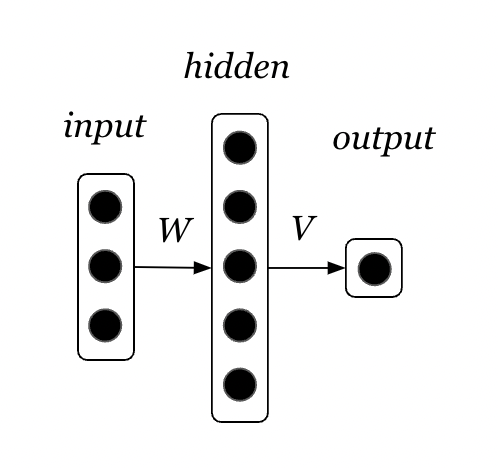
\includegraphics[width=0.3\textwidth]{images/fnn.png}
\caption{Example of a feedforward neural network}
\label{fig:fnn}
\end{figure}

\subsection{Recurrent Neural Network (RNN)}
Recurrent neural networks are usually used to deal with sequences. They allow access to the input data as well as past data to compute the next state. As shown in Figure \ref{fig:rnn}, the hidden layer $h_t$ is computed using both input $x_t$ at time $t$ and the hidden state $h_{t-1}$ which contains the history information from time 0 to $t-1$. For each timestep $t$, the hidden state can be expressed as:
\[ h_t = Wx_t + Uh_{t-1} \]

\begin{figure}[ht]
\centering
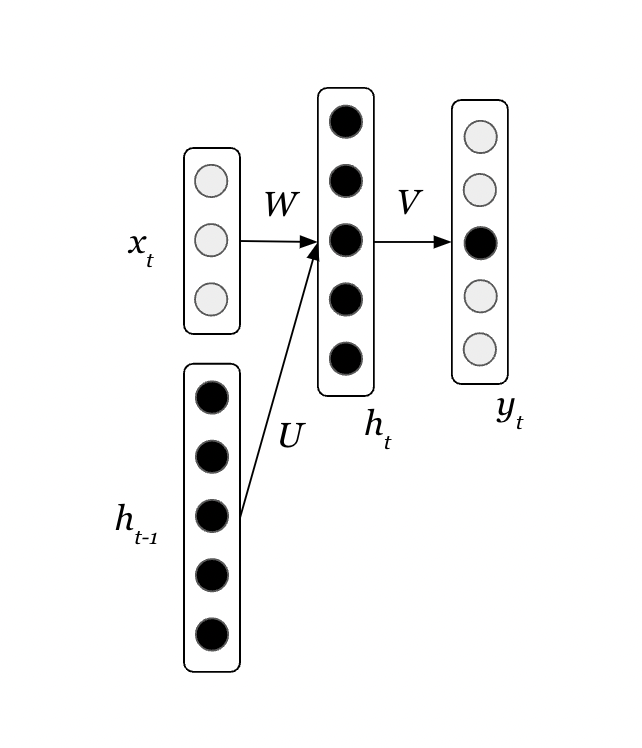
\includegraphics[width=0.4\textwidth]{images/rnn.png}
\caption{Example of a recurrent neural network (RNN)}
\label{fig:rnn}
\end{figure}


\subsection{Recursive Neural Network (RvNN)}
A recursive neural network has a tree-like structure. Figure \ref{fig:rvnn} illustrates an example of a basic RvNN architecture. The parent node representation is computed from its child nodes' representation as follows:
\[ p_{n, n+1} = f(W[x_n; x_{n+1}]) \]
where $f$ is the activation function. The same weight matrix $W$ will be applied recursively over the input.

\begin{figure}[ht]
\centering
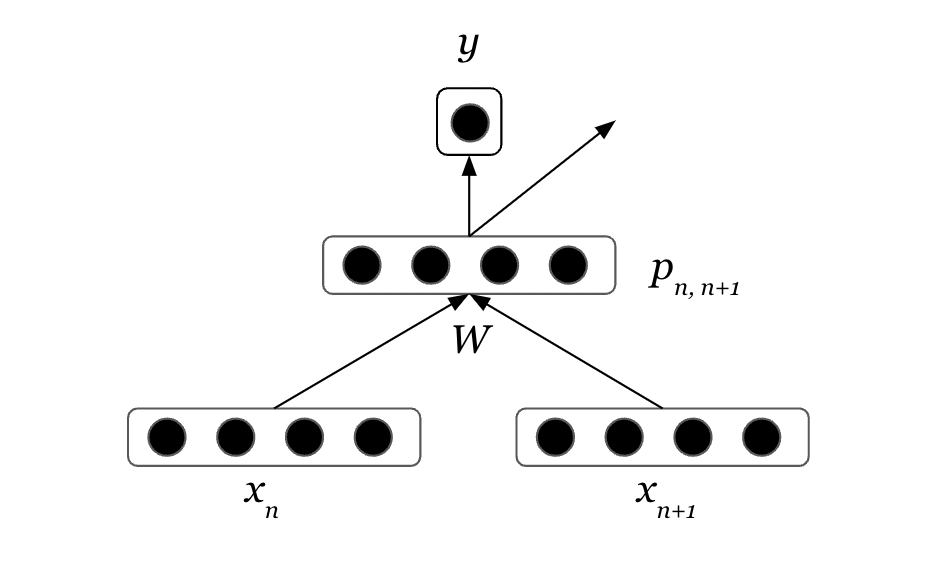
\includegraphics[width=0.6\textwidth]{images/rvnn.png}
\caption{Example of a recursive neural network (RvNN)}
\label{fig:rvnn}
\end{figure}


\subsection{\texorpdfstring{Recursive Recurrent Neural Network (R\textsuperscript{2}NN)}{Recursive Recurrent Neural Network (R2NN)}}
The R\textsuperscript{2}NN proposed by Liu et al.\cite{r2nn} combines the features of RvNN and RNN. It has a tree-like structure similar to RvNN, with recurrent vectors added to integrate global information. As shown in Figure \ref{fig:r2nn}, $s^{[l, m]}$ and $s^{[m, n]}$ is the representation of child nodes $[l, m]$ and $[m, n]$. The recurrent input vectors, $x^{[l, m]}$ and $x^{[m, n]}$ are added to the two child nodes respectively. They encode the global information, such as language model scores and distortion model scores. A third recurrent input vector $x^{[l, n]}$ is added to the parent node $[l, n]$. The parent node representation is computed as
\[ s_j^{[l, n]} = f(\sum_{i} \hat{x}_i^{[l, n]}w_{ji}) \]
where $\hat{x}$ is the concatenation of vectors $[x^{[l, m]}; s^{[l, m]}; x^{[m, n]}; s^{[m, n]}]$, and $f$ is the $HTanh$ function. The output, $y^{[l, n]}$, is computed as
\[ y^{[l, n]} = \sum_{j} ([s^{[l, n]}; x^{[l, n]}])_{j}v_j \]


\begin{figure}[ht]
\centering
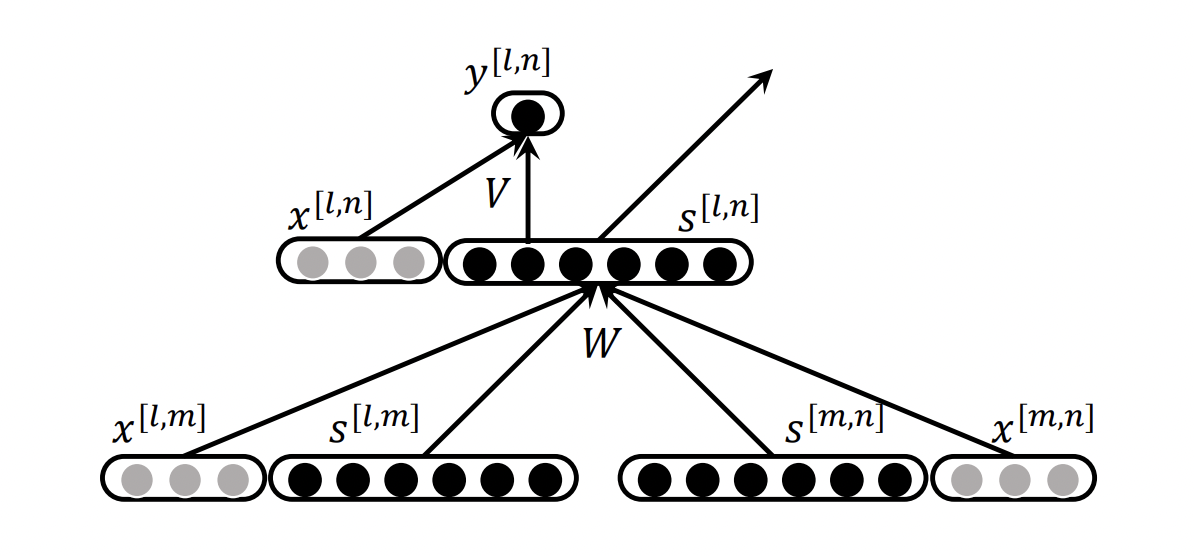
\includegraphics[width=0.6\textwidth]{images/r2nn.png}
\caption{Recursive recurrent neural network (Liu et al., 2014, p.1494)}
\label{fig:r2nn}
\end{figure}


\section{Requirement Analysis}

Based on the Project Structure section from my project proposal, the following requirements have been identified:

\textbf{Data preprocessing}
\begin{itemize}
    \item Data should be prepared in a form that is accepted by Moses SMT and R\textsuperscript{2}NN SMT
    \item Preprocessing should be done carefully to avoid accidentally correcting some of the grammatical errors 
    
    \begin{itemize}
        \item E.g. capitalisation errors may go undetected if all sentences are lowercased during data preprocessing
    \end{itemize}
\end{itemize}

\textbf{Moses SMT for GEC}
\begin{itemize}
    \item A language model should be trained to model the probability of a given sentence being valid
    \item A translation model should be trained to construct a phrase translation table
    \item A reordering model should be trained to learn the reordering of phrases
    \item With the above three models and Moses decoder, a complete Moses SMT system should be built
\end{itemize}

\textbf{R\textsuperscript{2}NN SMT for GEC}

Following the R\textsuperscript{2}NN paper by Liu et al.\cite{r2nn},
\begin{itemize}
    \item Phrase pair embeddings (PPE) should be learned by building a one-hidden-layer neural network and a recurrent neural network
    \item A recursive recurrent neural network (R\textsuperscript{2}NN) should be built and used as a decoder
\end{itemize}

\textbf{Evaluation}
\begin{itemize}
    \item The performance of both SMT systems should be evaluated using F0.5 scores
\end{itemize}

\section{Choice of Tools}

\subsection{Programming Language}

Python is chosen to be the main programming language as it provides many libraries that are commonly used for natural language processing. For this project I will be using \texttt{python 3.8} and PyCharm as my IDE.

\subsection{Libraries}
\textbf{PyTorch} \\
The \texttt{PyTorch}\footnote{https://pytorch.org/} library is one of the most popular machine learning frameworks. There are other similar libraries (such as \texttt{TensorFlow}) but I find \texttt{PyTorch} tutorials are easier to follow.

\textbf{NumPy} \\
My project is likely to involve statistical processing. I would be using the \texttt{NumPy}\footnote{https://numpy.org/} library for this purpose.

\textbf{pandas} \\
\texttt{pandas}\footnote{https://pandas.pydata.org/} is a powerful library for processing tabular data. This would be used to manipulate phrase tables in my project.

\subsection{Dataset}
The dataset introduced in BEA 2019 Shared Task\cite{bryant-etal-2019-bea} will be used in this project. I chose the two corpora (FCE v2.1 and W\&I+LOCNESS v2.1) which are immediately downloadable from the website\footnote{https://www.cl.cam.ac.uk/research/nl/bea2019st/\#data} to start with. The corpora have been standardised to be easily evaluated by ERRANT\cite{bryant-etal-2017-automatic,felice-etal-2016-automatic}. ERRANT is a toolkit used to annotate parallel data and compare hypothesis against reference to produce various evaluation metrics including F0.5 score. I may request other corpora as an extension of my project.

\subsection{Version Control and Backup}
Git will be used for version control. The entire project, including all the written code and my dissertation, will be pushed to GitHub regularly.

\chapter{Implementation}

\section{Repository Overview}
-

\section{Moses SMT}
-

\subsection{Pre-processing}
-

\subsection{Language Model}
-

\section{\texorpdfstring{R\textsuperscript{2}NN}{R2NN} SMT}
-

\subsection{Pre-processing}
-

\subsection{Phrase Pair Embedding}

\chapter{Evaluation}

\chapter{Conclusion}


%%%%%%%%%%%%%%%%%%%%%%%%%%%%%%%%%%%%%%%%%%%%%%%%%%%%%%%%%%%%%%%%%%%%%
% the bibliography
\addcontentsline{toc}{chapter}{Bibliography}
\bibliography{refs}

%%%%%%%%%%%%%%%%%%%%%%%%%%%%%%%%%%%%%%%%%%%%%%%%%%%%%%%%%%%%%%%%%%%%%
% the appendices
\appendix

\chapter{Project Proposal}

% \chapter{Latex source}

% \section{diss.tex}
% {\scriptsize\lstinputlisting[language=TeX]{diss.tex}}

% \section{proposal.tex}
% {\scriptsize\verbatiminput{proposal.tex}}

% \chapter{Makefile}

% \section{refs.bib}
% {\scriptsize\verbatiminput{refs.bib}}


% \chapter{Project Proposal}

% \input{proposal}

\end{document}